
\graphicspath{ {./content/rel/figure/} }

\section{Problem statement}\label{sec:2}

%%% \cite{moeininouvelle} - \cite{chin1988optimum} %%% exemple de citation 
 To find the best position of a set of cameras there are two key points.
The first key points is to develop an efficient algorithm to find best position for a rectangular room without any obstacle (like a wall or pylons) and all the cameras must be fixed on the ceiling toward the ground.
 	PSO is a computation method and try to optimize the problem by iteratively test. All step the algorithm takes the previous best solution and search a new set of solutions near to the best previous solution despite to the inertia. The inertia is a parameter to PSO using to limit the field of search on every step. 
The choice of PSO is appropriate to find the position of a camera for two main reasons.\\

-	Because is an optimization method and try to find the cameras positions is NP-hard and in this case you can find the optimal solution\\
-	PSO is already used on some paper for choosing the position of a set of camera  in certain condition \cite{zhou2011optimal,reddy2012camera}\\

The other key point is to qualify the quantity and the quality of the solution. For that it’s necessary to calculate the coverage of one camera. To estimate the coverage of one camera, it’s easier to use the pinhole model and a grid of points (presented at figure 2) and calculate what point is visible by one camera.

%% ajouté   fig1 algo.png 
%%Algorithm for calculate the cover of one camera with grid of the floor.  
\begin{figure}
  \centering
  \hspace*{\fill}
  %\subfigure[]{\label{subfig:4a}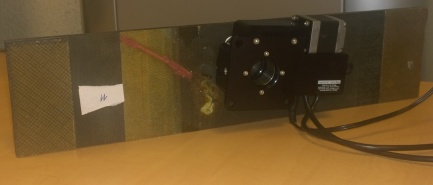
\includegraphics[width=0.3\linewidth]{fig4a.png}} \hfill
  %\subfigure[]{\label{subfig:4b}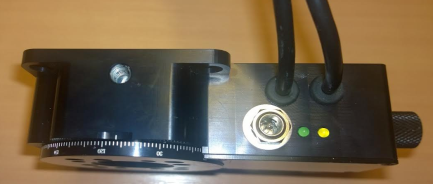
\includegraphics[width=0.3\linewidth]{fig4b.png}} 
  %\hspace*{\fill} \\ \hspace*{\fill}
  %\subfigure[]{\label{subfig:4c}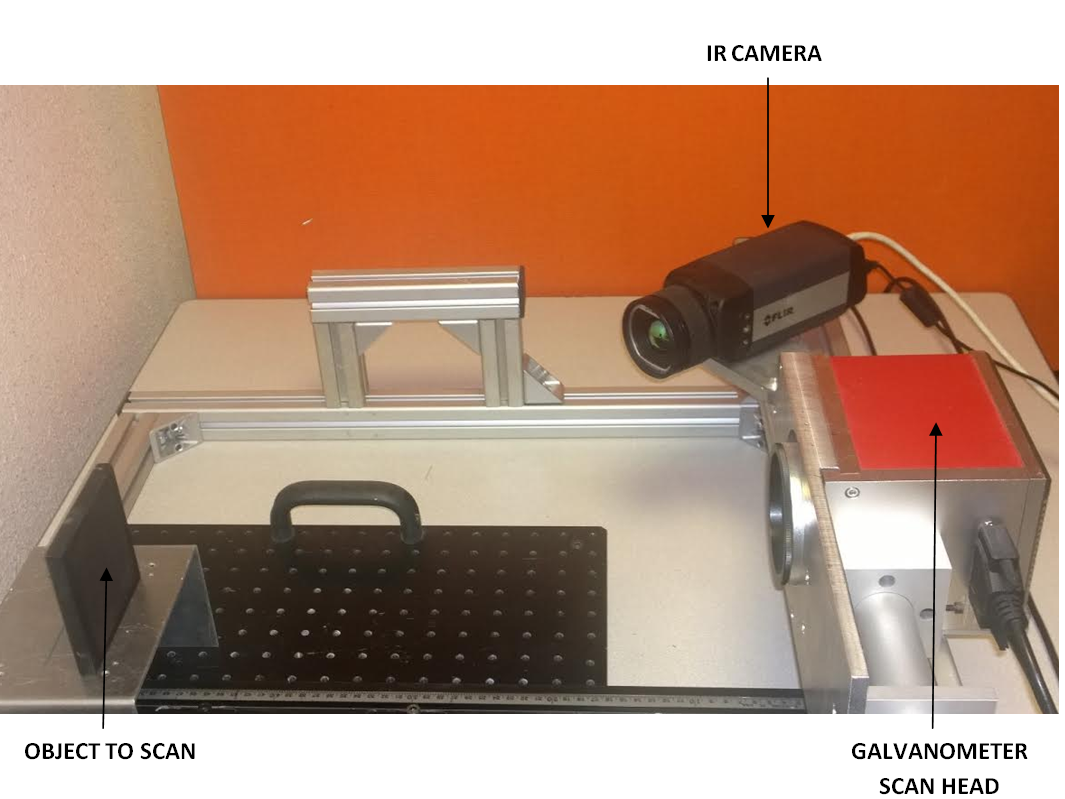
\includegraphics[width=0.3\linewidth]{fig4c.png}}
	.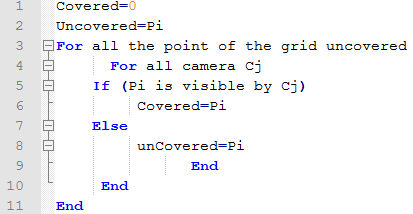
\includegraphics[width=0.7\linewidth]{algo.png}
  \hspace*{\fill}
  \caption{%(a)-(b) Device for positioning the composite material - 
	Algorithm for calculate the cover of one camera with grid of the floor.}
  \label{fig:422}
\end{figure}
%% ajouté   fig2 fig2.png 
%%Figure 2: Visualization grid with one camera coverage

\begin{figure}
  \centering
  \hspace*{\fill}
  %\subfigure[]{\label{subfig:4a}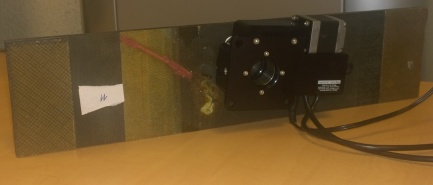
\includegraphics[width=0.3\linewidth]{fig4a.png}} \hfill
  %\subfigure[]{\label{subfig:4b}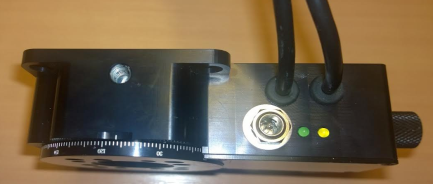
\includegraphics[width=0.3\linewidth]{fig4b.png}} 
  %\hspace*{\fill} \\ \hspace*{\fill}
  %\subfigure[]{\label{subfig:4c}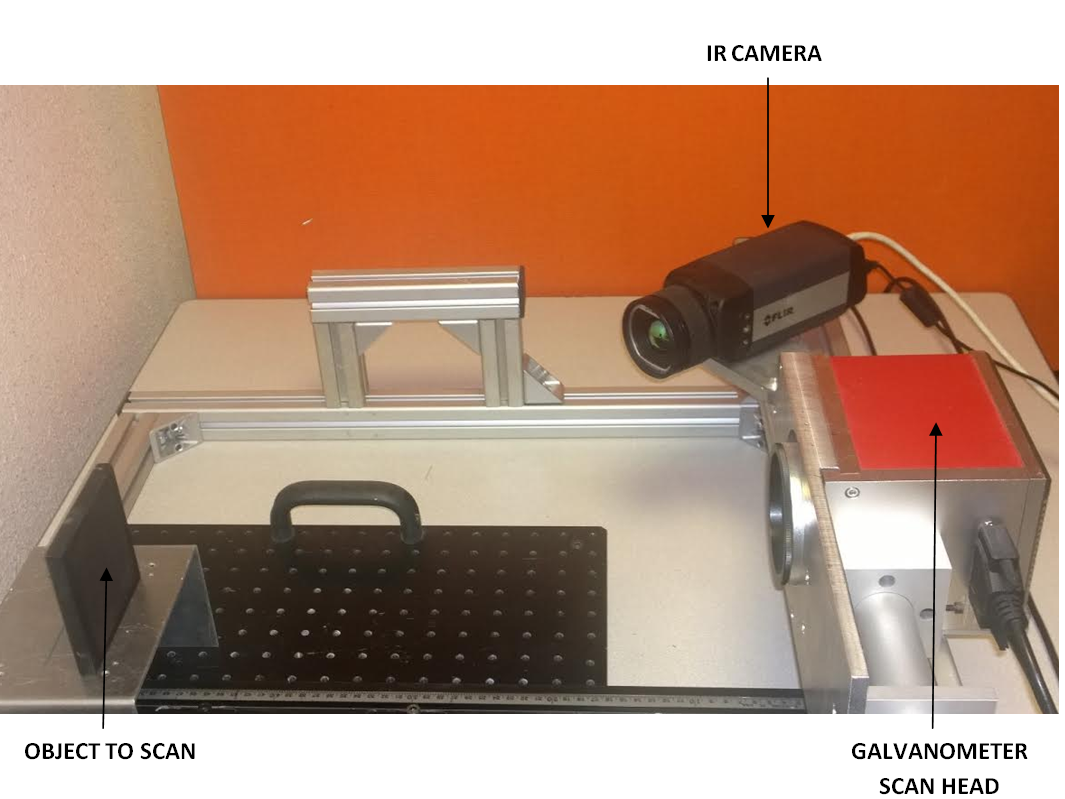
\includegraphics[width=0.3\linewidth]{fig4c.png}}
	.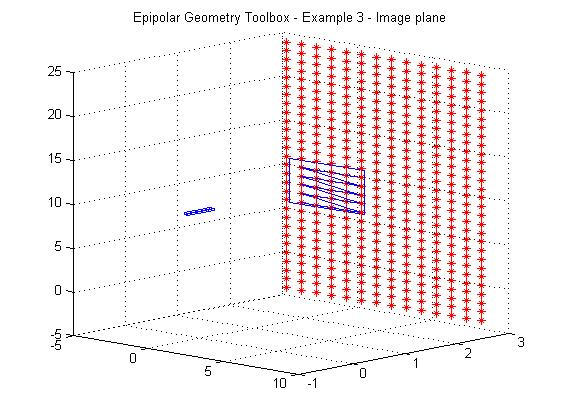
\includegraphics[width=0.7\linewidth]{fig2.png}
  \hspace*{\fill}
  \caption{%(a)-(b) Device for positioning the composite material - 
	 Visualization grid with one camera coverage.}
  \label{fig:422}
\end{figure}

To do this, it’s easier (and fast for computation) to use the pinhole camera model.  It’s necessary to put a grid of point on the floor and to any point it’s calculated if this point of the grid (figure 2) is covered by minimum one camera. Follow this algorithm, see (figure 1)


\subsection{Cost function for PSO and random walk }

When you know how to calculate the coverage of one camera. It’s possible to create one cost function to qualify the quality of the answer proposed by any kind of algorithm. 
The cost function is defined like below (1)
n= number of camera 
Grid = is a grid represent the floor. It’s used to calculate the coverage of a room\\
cover (n)=Coverage of the camera.\\
 $$ \text{Coverage rate of the room}= \sum\limits_{i=1}^{n}\frac{Cover(i)}{Size(grid)}text{(1)}$$



%%% Local Variables: 
%%% mode: latex
%%% TeX-master: "../../master"
%%% End: 
